\chapter{Assesing Avalanche problems }

%\section{Case Study}

In order to validate the performance of the avalanche problem algorithm the algorithm is applied to 
SNOWPACK simulations for one season (winter season 2021/22) driven by AWS within the EUREGIO. At first to the
AWS in the Axamer Lizum, which is well equiped and where we have regular field observations. For a bigger
picture the algorithm is tested on all 32 Asnowpack statioons for a critical situation with persitent weak layer 
especially north of the alpine main ridge. On addition the to simulations initialized by observed profiles and driven by NWPs
will be compared to the performance of the AWS simulations. As refference serve the issued avalanche problems by the local
avalanche warning service. 

\section{Overview Winterseason 2021/22} \label{sec:Results_overview}

\begin{figure*}[h]
    \centering
    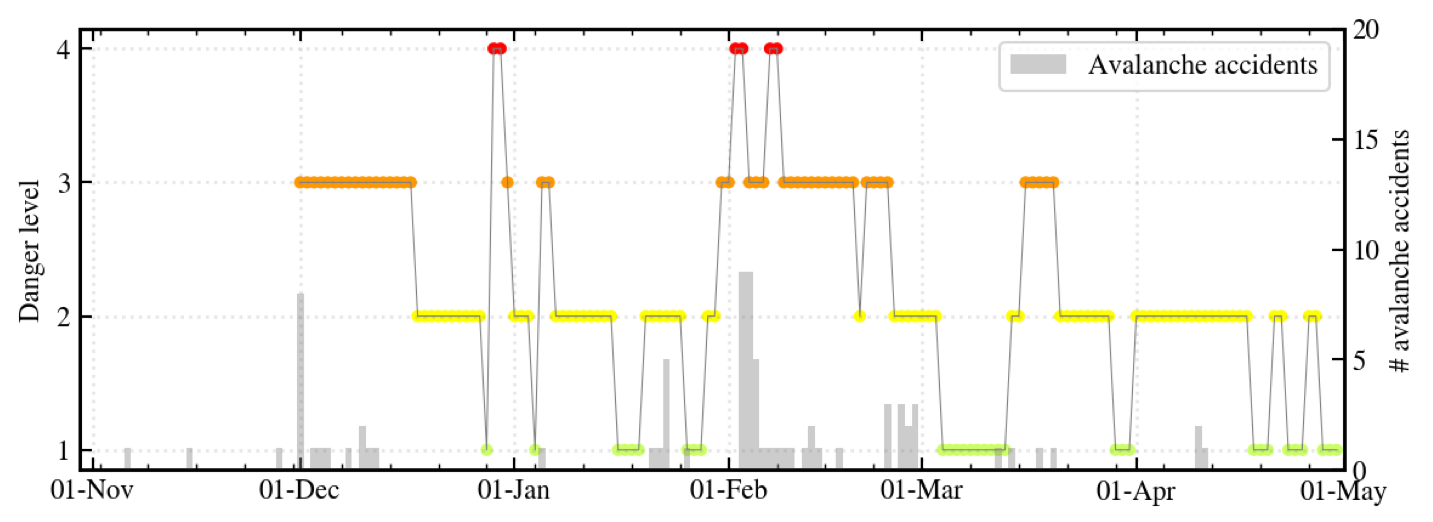
\includegraphics[width=0.8\textwidth]{Figures/figures_avapro/Dangerlevel_tirol.png}
    \caption{Evolution of the maximum avalanche danger level in tyrol in the winter season
     2021/22 and reported avalanche accidents with people involvment in the grey bars }
    \label{fig:dangerlevel_evolution}
\end{figure*}

\noindent Figure \ref{fig:dangerlevel_evolution} shows the evolution of the maximum avalanche danger level reachead in
 the winter season 2021/22 within the warning region of tyrol in the coloured dots. The danger level (DL) reaches from low-1 
 to high-4 DL. The grey bars indicate reported avalanche accidents where peopel where involved. Overall it was an average
 hazard evalution over the season showing two critical situations reaching high danger level. One at the end of december and
one in the beginning of feburary. Especially during the second phase a high ammount of avalnche accidents where reported. 




\section{Axamer Lizum} \label{sec:results_AXLIZ}

The Axamer Lizum is a ski resort nearby Innsbruck with a evaluation band from 1600m to 2600m. The tyrolian avalanche warning
service operates a well equipped weatherstation at a evaluation of 2103m. 

\begin{figure*}[h]
    \centering
    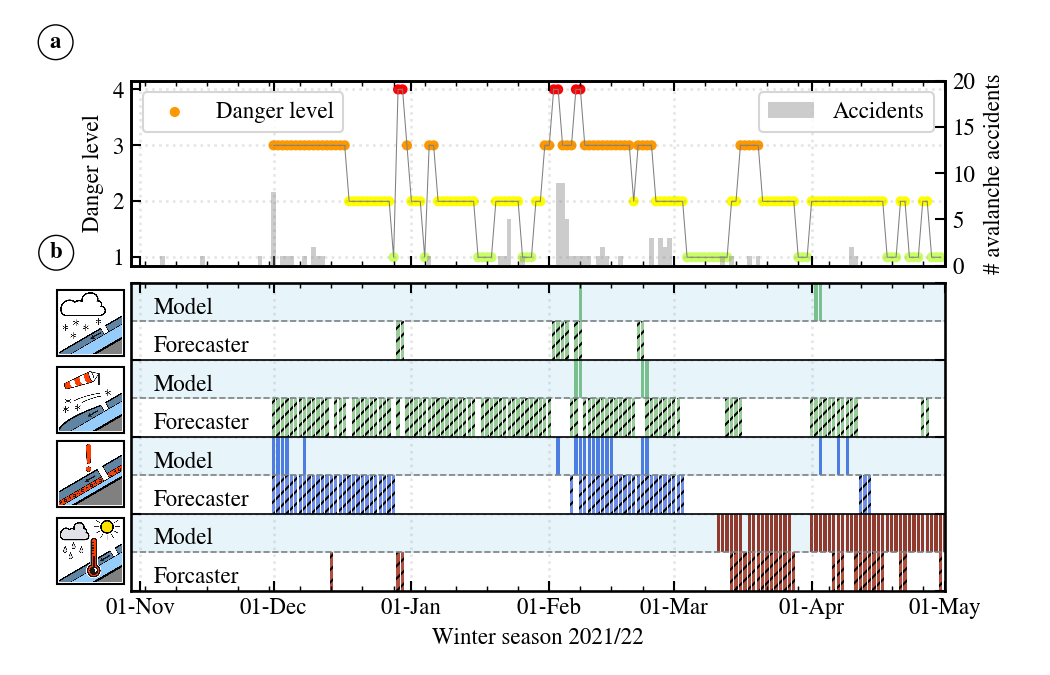
\includegraphics[width=0.8\textwidth]{Figures/figures_avapro/AXLIZ/AXLIZ_all.png}
    \caption{ a. Evolution of the maximum avalanche danger level in tyrol in the winter season
     2021/22 and reported avalanche accidents with people involvment in the grey bars \\
     b. Avalanache Problems Assigned by the model for all aspects in the blue shaded area and compared to the 
     problems assigned by the LWD for the region}
    \label{fig:avapro_AXLIZ_all}
\end{figure*}

\noindent Figure \ref{fig:avapro_AXLIZ_all}.a shows the evolution of the dangerlevel over the winterseason 2021/22 for the Axamer
Lizum in the coloured dots. (see \ref{sec:Results_overview}) Figure \ref{fig:avapro_AXLIZ_all}.b displays the avalanche problem
assignement for New Snow, Persitent weak layer and wet snow. For each of them is a blue shaded area wear bars indicate a relevant
problem assigned by the algorithm if any aspect is relevant. Below that a white area for avalanche problems assigned by the 
local avalanche warning service for that region of the Kalkkoegl (Axamer Lizum). Overall the model apears to have a fairly similar
behavior in assigning a problem than the problem assigned by the forecast, assigning similar problems in similar periods. Having a
deeper look into them there is a offset in the onset and the duration of a problem.



\subsection{New Snow}

-pipabu

\begin{figure*}[h]
    \centering
    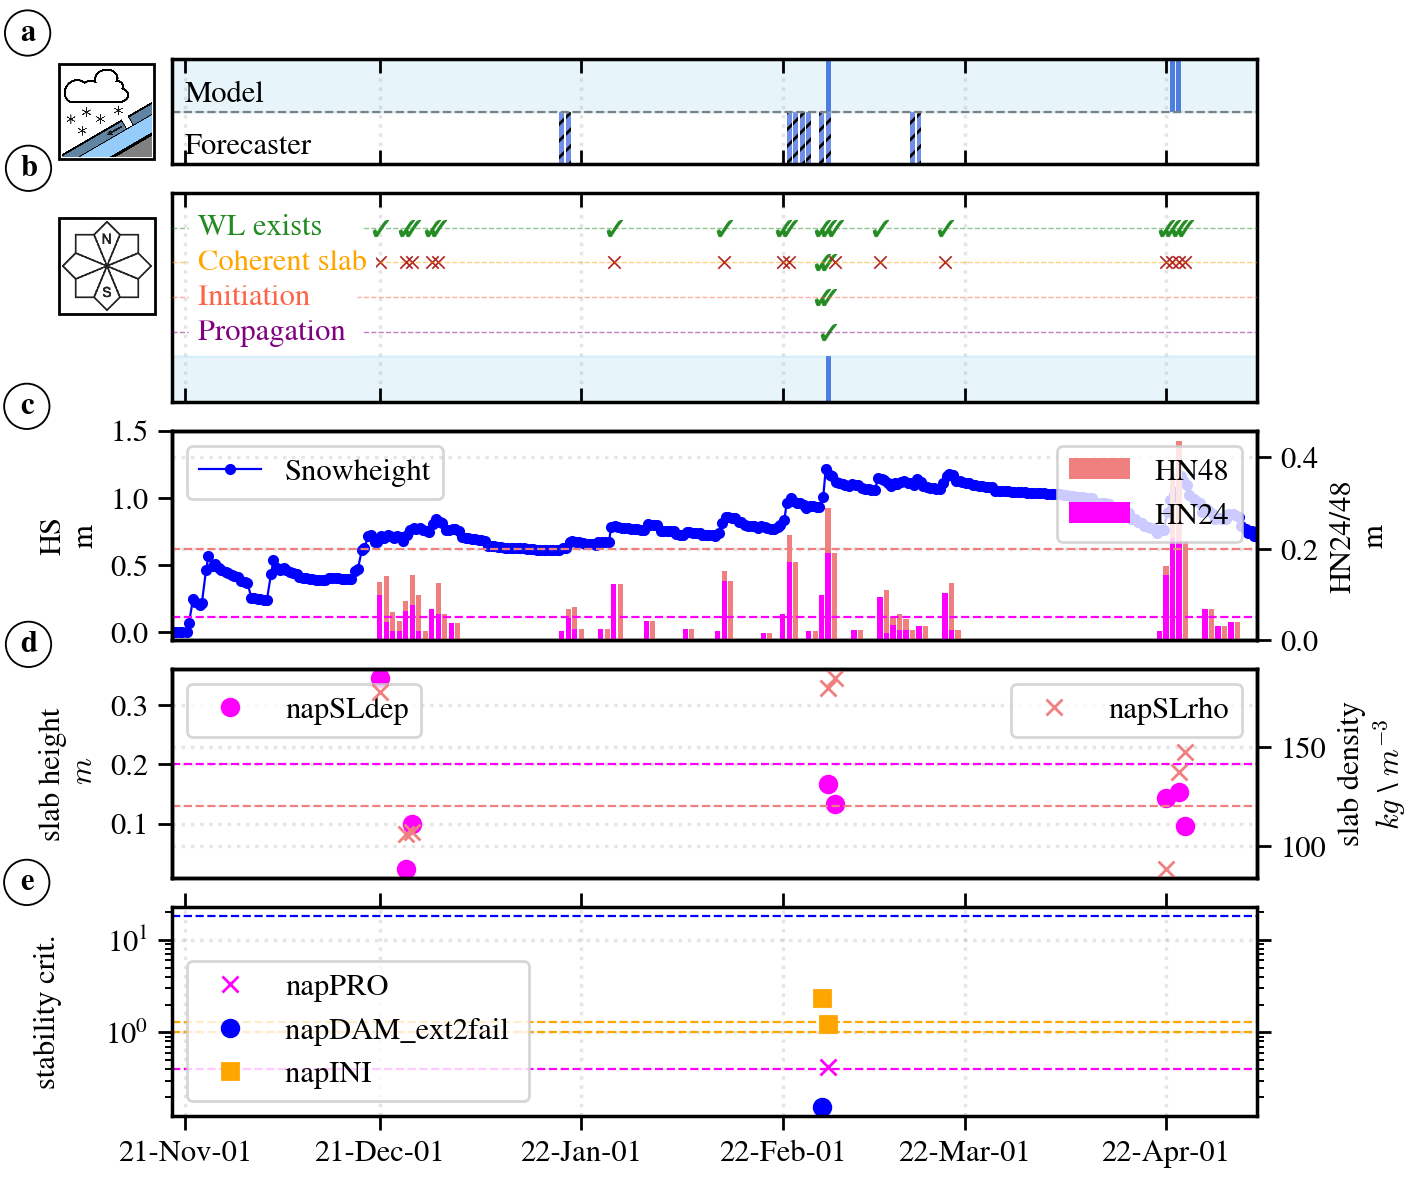
\includegraphics[width=0.8\textwidth]{Figures/figures_avapro/AXLIZ/new_snow_AXLIZ.png}
    \caption{New Snow Problem assesment for the flatfield simulationts driven by the AWS-Axamer Lizum Speicherteich}
    \label{fig:New_Snow_AXLIZ}
\end{figure*}

-pipabu \\
-pipabu\\
-pipabu\\
-pipabu\\
-pipabu\\
-pipabu\\


\subsection{Persistent Weak layer}

-mimmimi

\begin{figure*}[h]
    \centering
    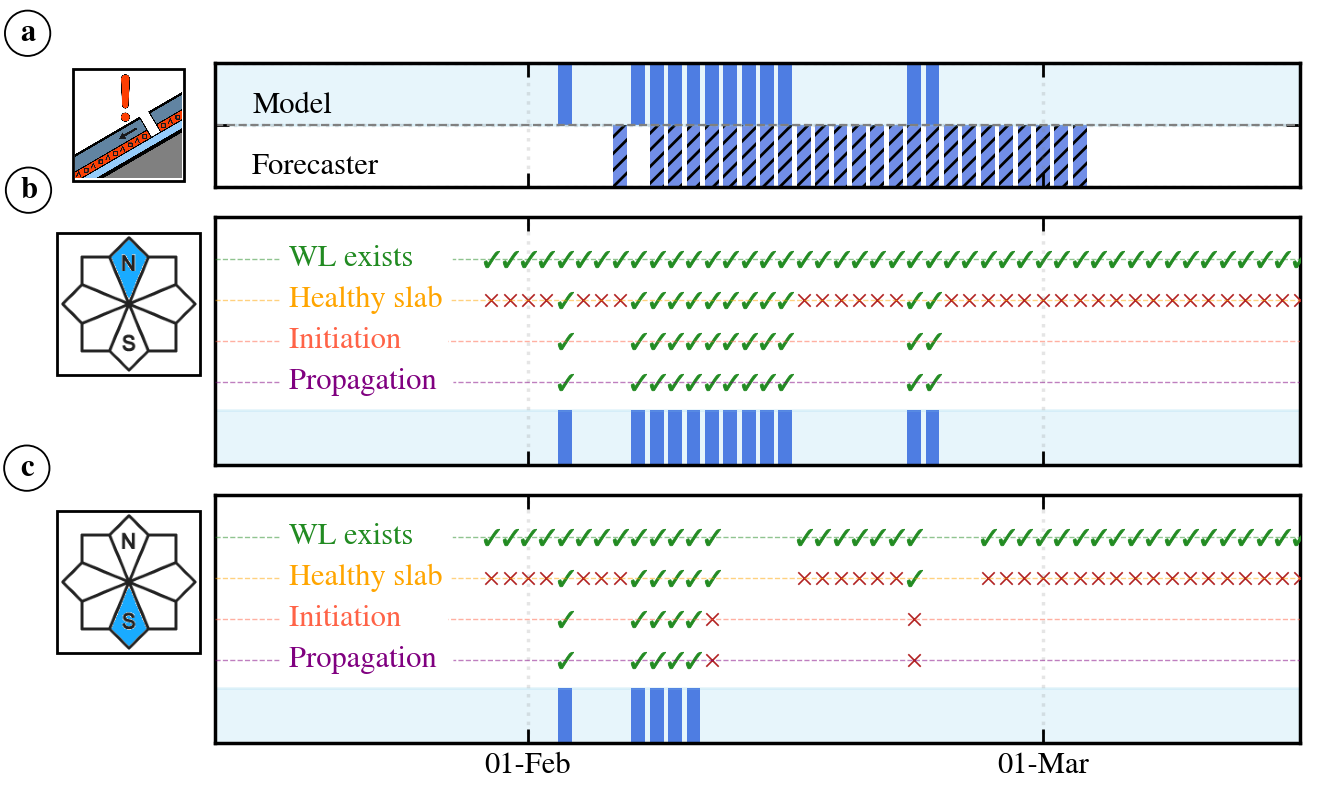
\includegraphics[width=0.8\textwidth]{Figures/figures_avapro/AXLIZ/persitent_N_S_AXLIZ.png}
    \caption{ (a.) Persisten weak layer assigned by the algorthim in the upper shaded area and assigned by the LWD Tyrol.
     (b.) Problem assesment for simulations for the northern aspect. (c.) Problem assesment for simulations for the southernn aspect.
     }
    \label{fig:PAP_N_S_AXLIZ}

\end{figure*}

blu bla bli

\begin{figure*}[h]
    \centering
    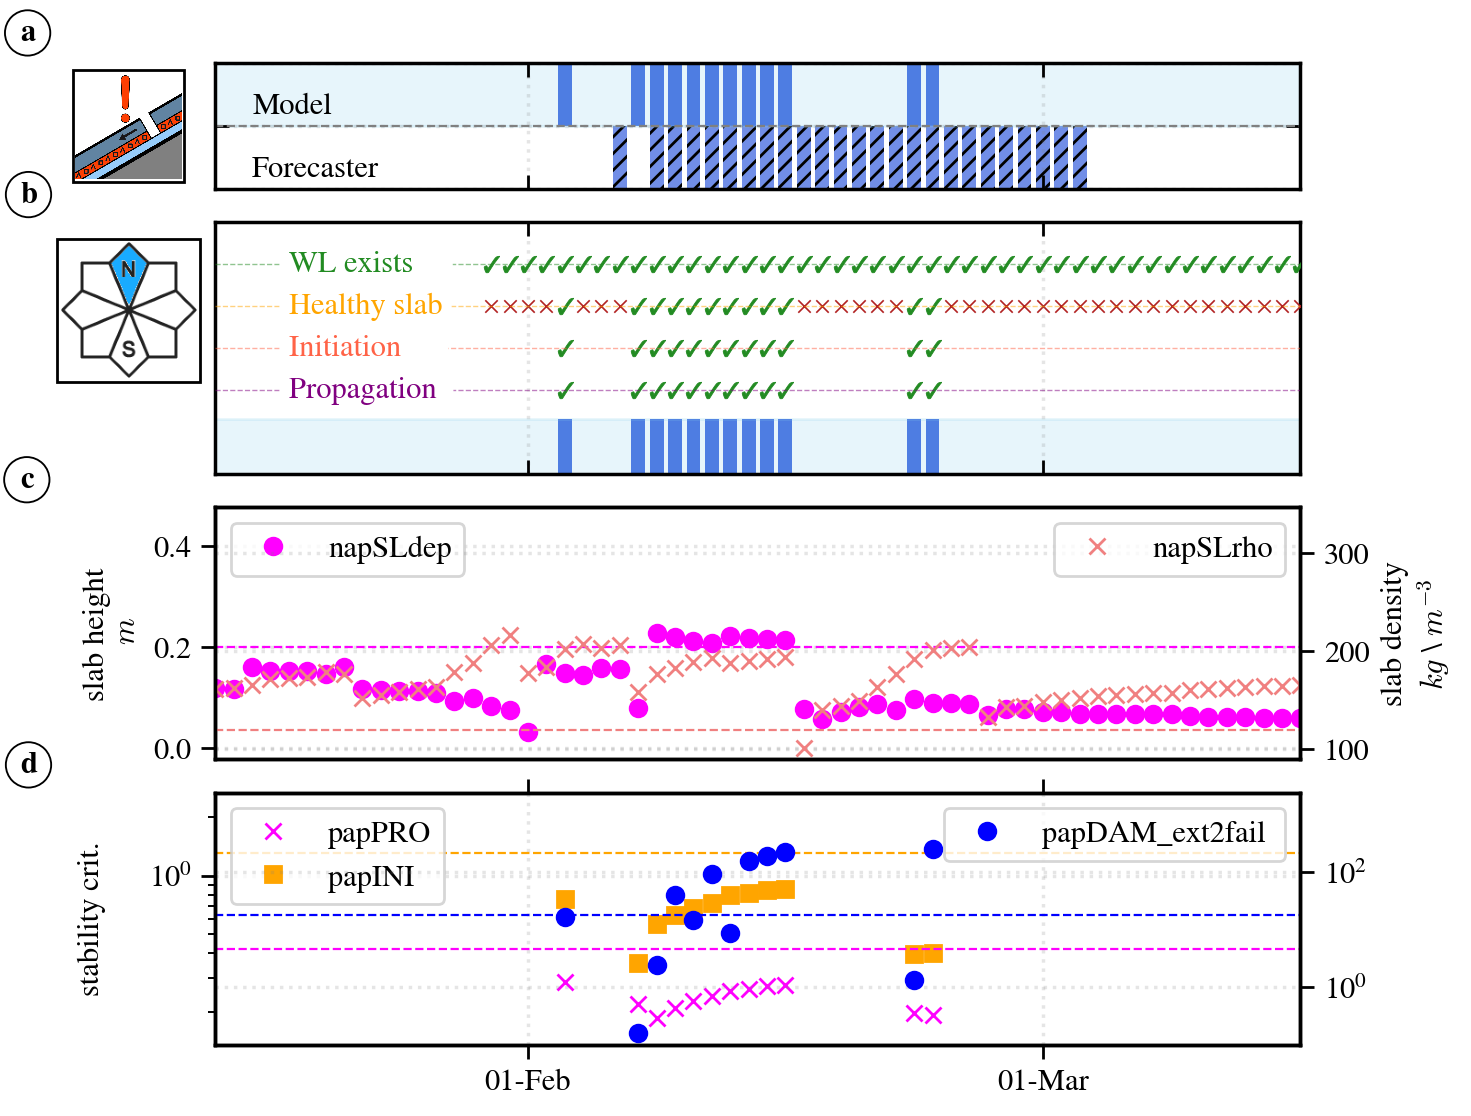
\includegraphics[width=0.8\textwidth]{Figures/figures_avapro/AXLIZ/persitent_N_detail_AXLIZ.png}
    \caption{ (a.) 
     (b.)(c.) 
     }
    \label{fig:PAP_N_detail_AXLIZ}

\end{figure*}



\subsection{Wet Snow}


\begin{figure*}[h]
    \centering
    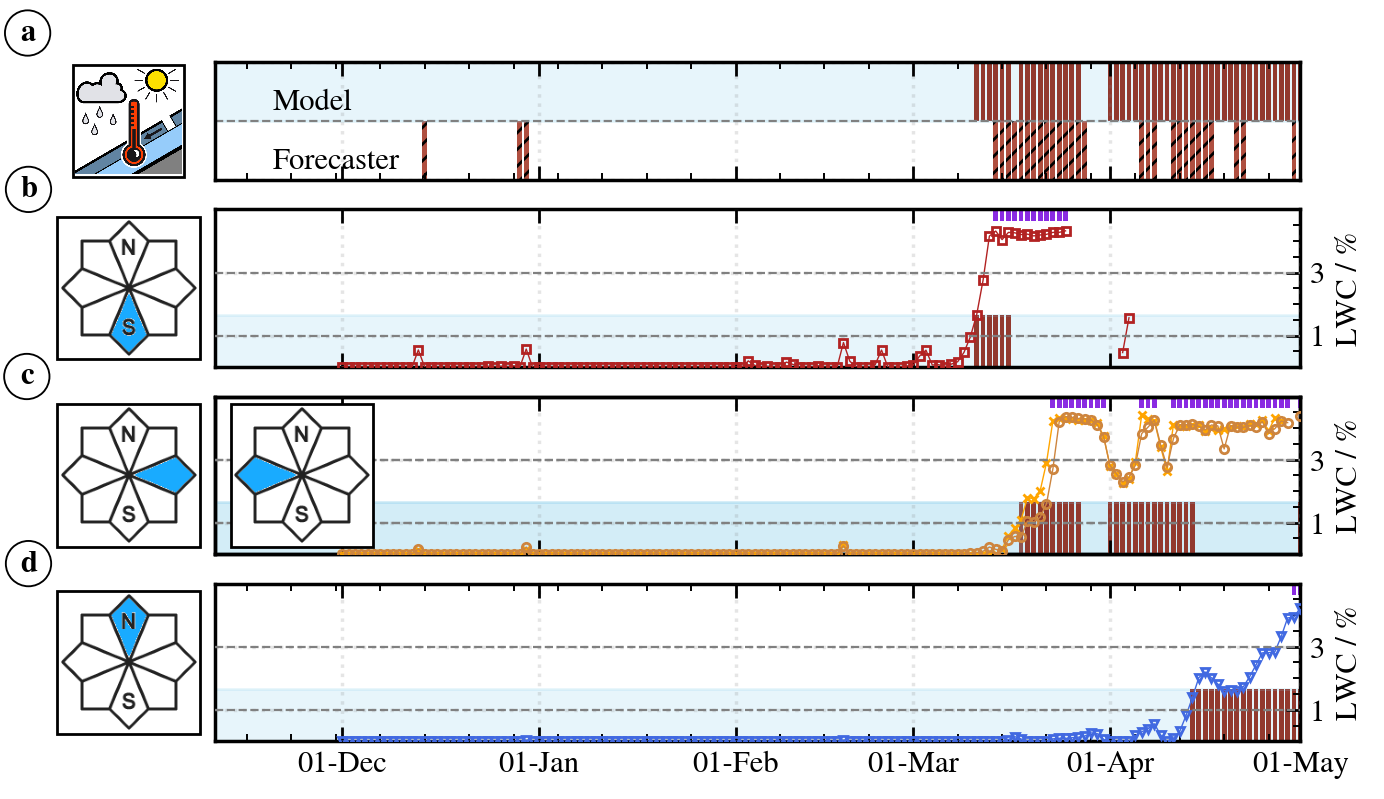
\includegraphics[width=0.8\textwidth]{Figures/figures_avapro/AXLIZ/wet_snow_AXLIZ.png}
    \caption{ a. Wet snow problem assigned by the algorthim in the upper shaded area, Wet snow problem assigned by the LWD Tyrol.  \\
     b. Wetsnowindx LWC for the snowpack simulations at the weatherstation Axamer Lizum Speicherteich for south- ($ \square$), 
     east- ($\times$),west- ($\circ$), north-($\bigtriangledown$) aspect, indication days of isothermal state in bars the respected
     upper corner and bars for a assigned problems in the lower part}
    \label{fig:avapro_AXLIZ_wet}
\end{figure*}

\noindent Figure \ref{fig:avapro_AXLIZ_wet} displays the  liquide water index LWC for the simulations for each aspect. The snowpack
reaches critical stability in the scope of the wet snow problem if the LWC-index exeeds a threshold of 1 (\cite{mittererOperationalSupportingTool2013})
the first time. Furthermore the instability exhibits several cycles if the LWC-index undershoots and overshoots a value of 3 (\cite{mittererOperationalSupportingTool2013}).
If so a wet snow problem is assigned. The conditions stays unstabel as long as 4 days of isothermal state of the snowpack (see \ref{sec:methods_wetsnow}).

The simulations of the southern aspect reaches the critical threshold first in the beginning of March, but as well reaches a isothermal state off
more than 4 days to be in a stable condition again. Followed by the eastern and western aspect more ore less simultaniously. The east and west slopes
undergoe sevaral cycles till the end off the season. At last the northern aspects reaches the LWC-index to become a wetsnow problem. 

The increase of the LWC within the snowpack can be due to radiation, temperature increase and addidinonal water input due due liquid percipitation.
Rain on snow affects all aspects in the same well. The southern aspects suffer from the best angle to the sun and the highest temperature within the 
daily cycle. 

What kind of a funny finding is that althoug the southern aspects gets critical at first they also reaches stability again due to no additional cycles.
More unpredictable are the eastern and western slopes. With stronger daily cycles and therefore wetsnow cycles. Northern aspects got critical at the 
end of the season to overall high temperatures.

Comparering  problem assignement

Phase in Dec

\subsection{Wind drift}

- mimimi funtz nit 


\begin{figure*}[h]
    \centering
    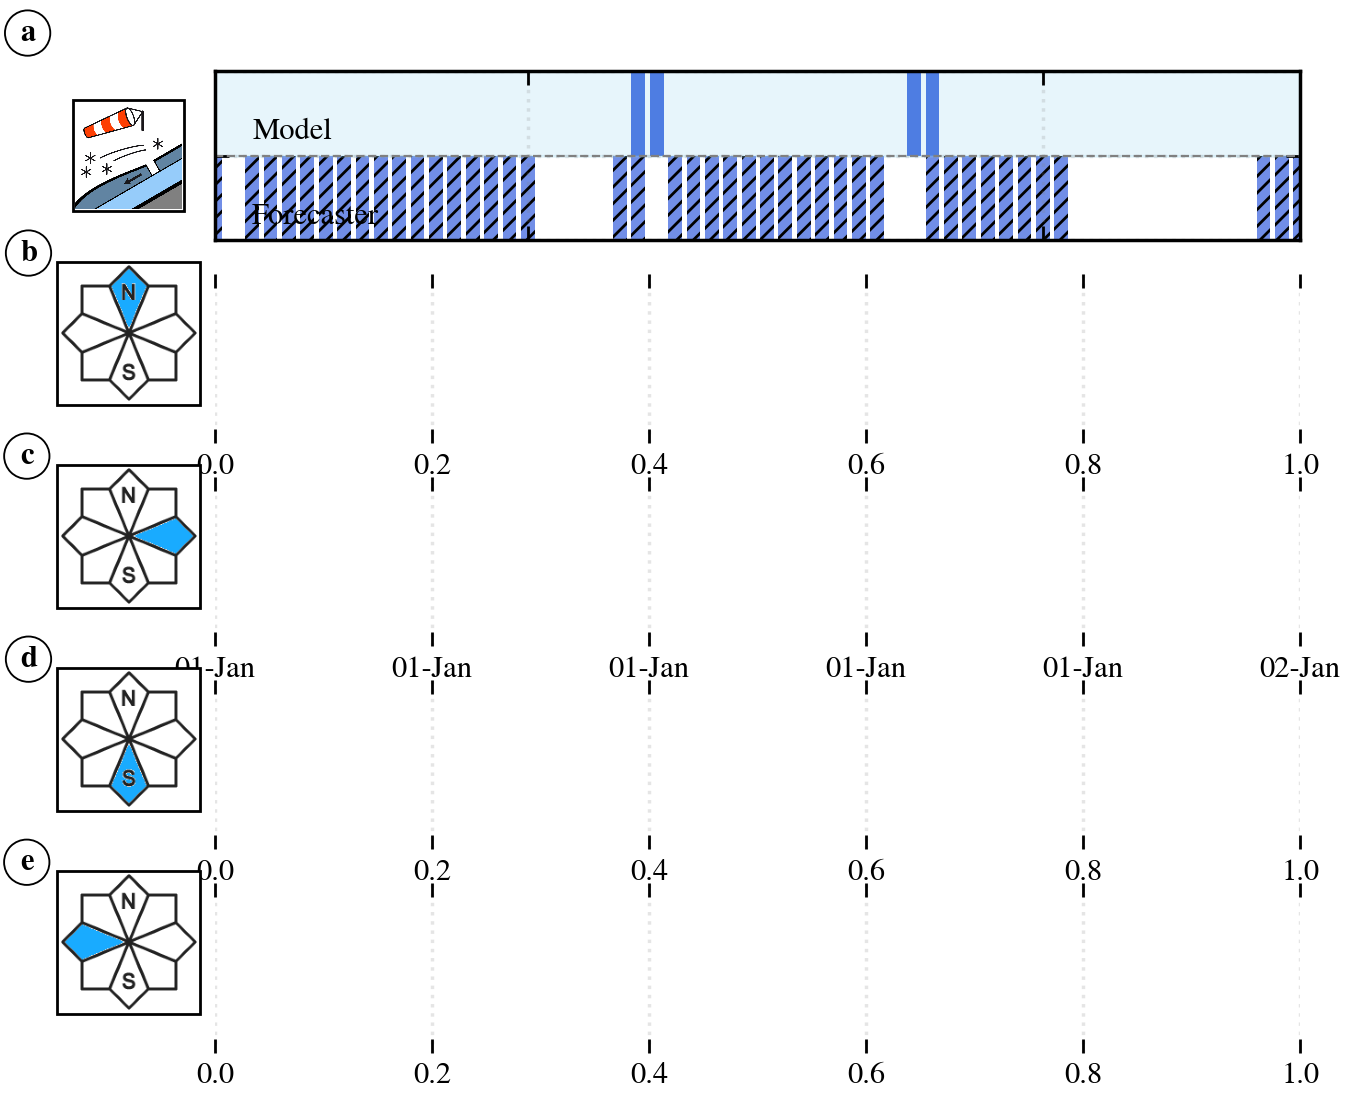
\includegraphics[width=0.8\textwidth]{Figures/figures_avapro/AXLIZ/winddrift_AXLIZ.png}
    \caption{winddrift}
    \label{fig:AWS_vs_NWPS}
\end{figure*}

\section{AWS vs observed Profile NWPs}

\begin{figure*}[h]
    \centering
    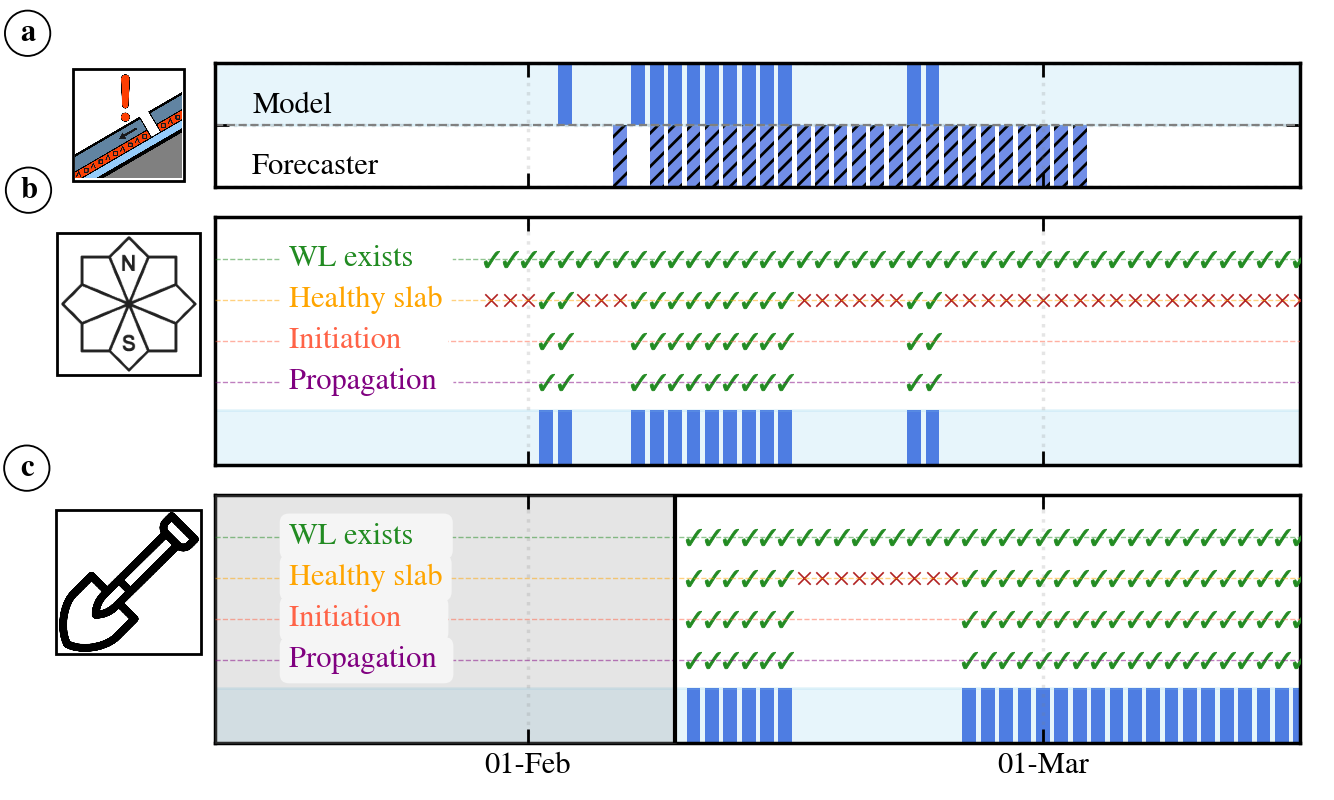
\includegraphics[width=0.8\textwidth]{Figures/figures_avapro/AXLIZ/persitent_profile_comp.png}
    \caption{Avalanche Problem assigmend of the flat field simulations driven by AWS 
    and initialized by a observed profile and driven by NWPS}
    \label{fig:AWS_vs_NWPS}
\end{figure*}

\noindent Figure \ref{fig:AWS_vs_NWPS} shows a the problem assigment for a persitent weak layer for the simulations driven by the AWS (b)
and the simulations initialized by a observed profile and driven by NWPs (c). In the uppermost plot (a) is the comparison of the modell
assesment to the local  avalanche warning service for the period of feburary til end of March. The black bar in (c) indicates the day of 
the profile observation from that day on it is driven by a 24 hour stacked forecast. The simulations driven by the AWS (b) are for the flat
field. The profile is aswell digged in the flat field nearby the weather station. 

\noindent Both simulations are showing the same behaviour for assigning the persitent weak layer especially for the first period. In both cases the
problem is not characterized as relevant after the 6th day case there is no coherent slab above the weak layer suporting crack propagation
and initiation. As the forecasting time increases (>10 days) the reassignment of the problem assignment differs. The AWS-simulations
reassign the problem a few days earlier than the NWP simulations, detecting a coherent slab, just to dropp it after the 2nd day. 
The offset can be due to the circumstance the the AWS-simulations are a nowcast. Only input parameters realy measuret at a day are taken into
account. Althoug a 24h leadtime forecast shows relativly precice forecast data it is still a forecast. Forecasted events might or might not 
happen. Therefore a forecasted event which is not happening will lead to a different snowpack cover. 

\noindent This is quite good news for avalanche warning services not having a big coverage of weather stations. Furthermore spatial information 
gaps can be reduced to simulations driven by NWPs. It will deliver a great opertunity to observe areas before a weather change (as an upcoming front)
and then simulate the snowpack from that day on. 



\section{ vrgl stations nord /south hauptkamm}


- signifikanter cut nördlich südlich alpenhauptkamm\\
- LWD übersicht\\
- zeigen stationen ähnliches verhalten
\begin{figure*}[ht]
    \centering
    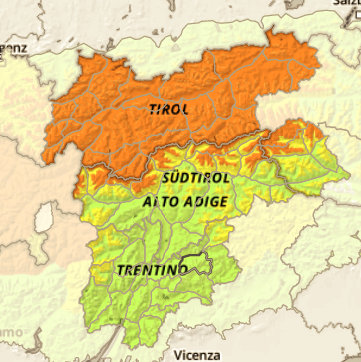
\includegraphics[width=0.8\textwidth]{Figures/figures_avapro/station_comp/report_feb_pap.png}
    \caption{Avalanche bulletin Euregio 04.Feb }
    \label{fig:ava_report_feb}
\end{figure*}

\begin{figure*}[ht]
    \centering
    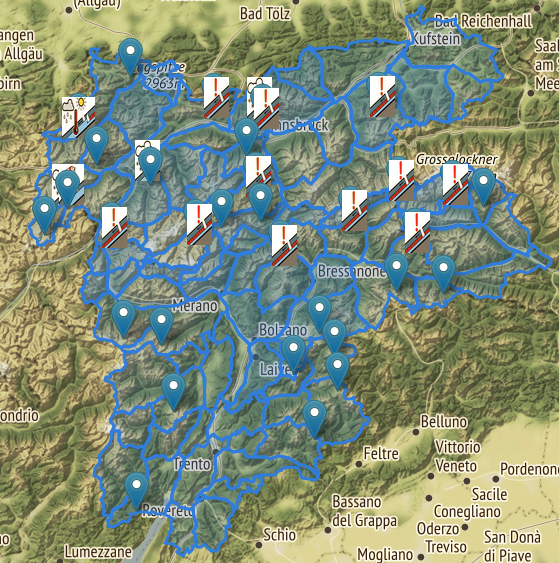
\includegraphics[width=0.8\textwidth]{Figures/figures_avapro/station_comp/station_comp_2022_02_04.png}
    \caption{Locations of the operation Snowpackstations within the EUREGIO}
    \label{fig:Snowpackstations_eruegio}
\end{figure*}

